% 1977 年宁夏卷第 10 题：三角形 ABC（A 在上方），AD 为 BC 边上的垂线，D 为垂足（按源卷第 2 页布局）
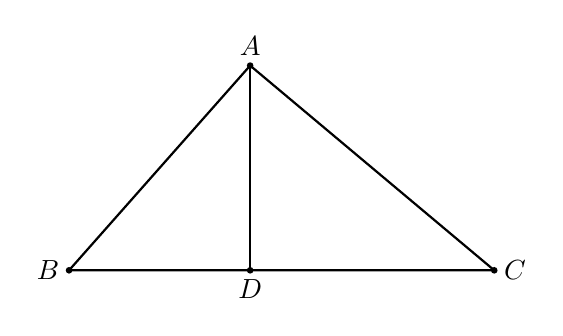
\begin{tikzpicture}[scale=1.0]
  \coordinate (A) at (2.3,2.6);
  \coordinate (B) at (0,0);
  \coordinate (C) at (5.4,0);
  \coordinate (D) at (2.3,0);
  \draw[thick] (B)--(C)--(A)--cycle;
  \draw[thick] (A)--(D);
  \fill (A) circle (1.2pt) node[above] {$A$};
  \fill (B) circle (1.2pt) node[left] {$B$};
  \fill (C) circle (1.2pt) node[right] {$C$};
  \fill (D) circle (1.2pt) node[below] {$D$};
\end{tikzpicture}
